\subsection{Module 7: Các chức năng về nhắn tin cho khách thuê}
\subsubsection{User stories}
\begin{itemize}
    \item Khách thuê có thể nhắn tin cho chủ nhà để hỏi thêm thông tin về phòng ốc, điều kiện phòng, ...
    \item Khách thuê có thể nhận và đọc phản hồi từ chủ nhà.
    \item Khách hàng có thể trả lời tin nhắn của chủ nhà.
    \item Khách hàng có thể xoá tin nhắn.
\end{itemize}

% ########################################################
\begin{figure}[!h]
	\centering
	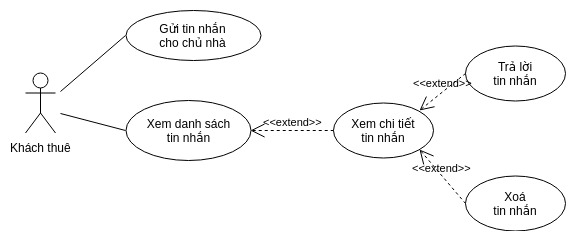
\includegraphics[width=\textwidth]{parts/Cuong/images/module5b.jpg}
	\caption{Lược đồ use case của module 5a: Các chức năng về nhắn tin cho khách thuê}
\end{figure}


% ########################################################
\subsubsection{Các use case chi tiết}

\subsubsubsection{Gửi tin nhắn cho chủ nhà}
\begin{usecase}
    \usecasename{Gửi tin nhắn cho chủ nhà}
	\actor{Khách thuê}
	\describe{Khách thuê xem danh sách tất cả tin nhắn đã nhận từ chủ nhà}
	\creators{Văn Tiến Cường}{Văn Tiến Cường}
	\datecreated{30/03/2019}{30/03/2019}
	\precond{Khách thuê đang ở trang thông tin phòng}
	\postcond{Tin nhắn được gửi đi và hệ thống gửi thông báo thành công}
	\normalflow
	\begin{enumerate}
		\item Khách thuê chọn \textbf{Gửi tin nhắn cho chủ nhà}.
        \item Hệ thống hiện cửa sổ soạn tin nhắn
        \item Người dùng nhập nội dung tin nhắn.
        \item Người dùng chọn nút \textbf{Gửi tin nhắn}
        \item Hệ thống gửi tin nhắn và thông báo thành công.
	\end{enumerate} \\ \hline
	
	\altflow
	\begin{itemize}
		\alt{2a} Người dùng chưa đăng nhập vào hệ thống.
		\begin{enumerate}
		    \item Hệ thống chuyển người dùng đến chức năng \textbf{Đăng nhập}.
		    \item Người dùng thực hiện chức năng \textbf{Đăng nhập}.
		    \item Hệ thống tiếp tục thực hiện từ bước 3.
		\end{enumerate}
	\end{itemize} \\ \hline
	
	
	\noexception
\end{usecase}


\subsubsubsection{Xem danh sách tin nhắn}
\begin{usecase}
    \usecasename{Xem danh sách tin nhắn}
	\actor{Khách thuê}
	\describe{Khách thuê xem danh sách tất cả tin nhắn đã nhận từ chủ nhà}
	\creators{Văn Tiến Cường}{Văn Tiến Cường}
	\datecreated{30/03/2019}{30/03/2019}
	\precond{Khách thuê đã đăng nhập thành công}
	\postcond{Hệ thổng hiển thị danh sách các tin nhắn được gửi cho khách thuê}
	\normalflow
	\begin{enumerate}
		\item Khách thuê chọn mục \textbf{Tin nhắn}.
        \item Hệ thống hiện ra danh sách tin nhắn với gồm các trường \textbf{Người gửi}, \textbf{Thời gian gửi}. \textbf{Chủ đề}
	\end{enumerate} \\ \hline
	
	\noalternative
	\noexception
\end{usecase}

\subsubsubsection{Xem chi tiết tin nhắn}
\begin{usecase}
    \usecasename{Xem chi tiết tin nhắn}
    \actor{Khách thuê}
    \describe{Khách thuê xem chi tiết một tin nhắn trong danh sách tin nhắn đã gửi cho mình}
    \creators{Văn Tiến Cường}{Văn Tiến Cường}
	\datecreated{22/03/2019}{30/03/2019}
    \precond{Khách thuê đang xem danh sách tin nhắn}
    \postcond{Hiện thông tin chi tiết về tin nhắn được Khách thuê chọn xem}
    
    \normalflow
	\begin{enumerate}
        \item Khách thuê chọn một tin nhắn trong danh sách tin nhắn.
        \item Hệ thống hiển thị tin nhắn cho Khách thuê, gồm các trường \textbf{Người gửi}, \textbf{Thời gian gửi}, \textbf{Chủ đề}, \textbf{Nội dung tin nhắn}, \textbf{Trạng thái đặt phòng}.
    \end{enumerate} \\ \hline
        
    \noalternative
    \noexception
\end{usecase}

\subsubsubsection{Trả lời tin nhắn}
\begin{usecase}
    \actor{Khách thuê}
    \describe{Khách thuê trả lời cho một tin nhắn đã gửi cho mình}
    \creators{Văn Tiến Cường}{Văn Tiến Cường}
	\datecreated{22/03/2019}{30/03/2019}
    \precond{Khách thuê đang xem chi tiết một tin nhắn nào đó}
    \postcond{Hệ thống gủi tin nhắn phản hồi tới cho khách thuê và thông báo thành công}

    \normalflow
	\begin{enumerate}
        \item Khách thuê chọn nút \textbf{Trả lời}.
        \item Khách thuê nhập nội dung phản hồi.
        \item Khách thuê chọn nút \textbf{Gửi}.
        \item Hệ thống thông báo tin nhắn gửi thành công.
    \end{enumerate} \\ \hline
        
    \noalternative
    
    \exception
    \begin{itemize}
        \alt{3a} Khách thuê chọn \textbf{Huỷ}. Hệ thống sẽ huỷ tin nhắn hiện tại và trở về hiển thị tin nhắn chi tiết.
    \end{itemize} \\ \hline
\end{usecase}


\subsubsubsection{Xoá tin nhắn}
\begin{usecase}
    \actor{Khách thuê}
    \describe{Khách thuê xoá một tin nhắn đã chọn}
    \creators{Văn Tiến Cường}{Văn Tiến Cường}
	\datecreated{22/03/2019}{30/03/2019}
    \precond{Khách thuê đang xem chi tiết một tin nhắn nào đó}
    \postcond{Tin nhắn được chọn bị xoá và hệ thống hiện thông báo xoá thành công}
    
    \normalflow
    \begin{enumerate}
		\item Khách thuê chọn nút \textbf{Xoá}.
        \item Hệ thống yêu cầu xác nhận xoá.
        \item Khách thuê chọn \textbf{Đồng ý}.
        \item Hệ thống thông báo xoá tin nhắn thành công.
	\end{enumerate} \\ \hline
	
	\noalternative
    
    \exception
    \begin{itemize}
        \alt{3a} Khách thuê chọn \textbf{Huỷ}. Hệ thống sẽ huỷ tin nhắn hiện tại và trở về hiển thị tin nhắn chi tiết.
    \end{itemize} \\ \hline
\end{usecase}